\chapter{Diffusion Approximation}
\label{chapter:da}

\section{Parametrization}
Artists prefer to define surface albedo and mean multiple scattering distance
(characteristic or visible depth of the SSS). The radiative transport scattering
coefficients must therefore be inferred by inverting the diffusion equation.
Test: as seen at the figure \ref{fig:dragon_ptdl} at page \pageref{fig:dragon_ptdl}

The scattering was parameterized by the volume scattering and absorption
coefficients $\sigma_s$ and $\sigma_a$ (or, equivalently, the volume
scattering albedo $\alpha = \sigma_s/\sigma_t = \sigma_s/(\sigma_s + \sigma_a)$
and volume mean free path length $l = 1/\sigma_t = 1/(\sigma_s + \sigma_a)$.)
In follow-up work, Jensen and Buhler \cite{Jensen:2002:RHR:566570.566619}
introduced a more intuitive parameterization of subsurface scattering:
surface albedo (diffuse surface reflectance) $A = \int\limits_0^\infty
R(r)2\pi r dr$ and diffuse mean free path length $l_d$ on the surface.

Such "albedo inversion" must typically done with iterative or tabulated methods,
both of which can have trouble with high albedos. Another challenge is that
diffusion profiles are often too blurry given that they typically only model
multiple scattering, leading to the use of two or more profiles combined in an
ad hoc manner.


\section{Christensen-Burley method}
The general problem discussed here is a search for a good diffusion
approximation model to fit Monte Carlo references by using analytic BSSRDF function.

The most recent research in this topic up to date
\cite{Christensen:2015:ARP:2775280.2792555}, \cite{Burley:disney_siggraph15}
suggested the \gls{BSSRDF} profile expressed as a combination of two exponential
functions with corresponding parametrization factor based on physical properties
of the media and proper normalization to ensure energy conservation. It was
proposed as function which better fit Monte Carlo references than widely used
Gaussian and Cubic profiles.

The original proposed diffuse reflectance profile:
\begin{equation}\label{eq:burley}
R_{l=1}(r) = As\dfrac{e^{-sr}+e^{-sr/3}}{8\pi r}
\end{equation}
With:
\begin{itemize}
    \item{$r$ is a distance between the points of light, entering and leaving
    the surface (with the assumption of the planar geometry)}
    \item{$s$ is a function of $A$, empirically chosen by Christen and Burley
    to fit the Monte-Carlo references. For example, for the Searchlight
    scenario, authors suggest $s = 1.85 - A + 7|A-0.8|^3$}
    \item{ $A=\int_0^{\infty} R(r)2\pi rdr$ is the surface albedo (integral
    amount of the radiant exitance over whole area of the object relative to the
    overall irradiance). Surface albedo of the material depends on $\sigma_s$
    and $\sigma_a$. The particular form of this function, empirically chosen by
    Christen and Burley to fit the Monte-Carlo references.}
\end{itemize}

In contrast to the other diffusion approximation techniques proposed in the past
(Dipole, Quantized diffusion), this model already includes single scattering
component, so no expensive separate calculation is needed.


According to the authors, the main disadvantages of the model are:
\begin{itemize}
  \item {As all other Diffusion approximation models, it still follows the
  infinite plane geometry assumption
  }
  \item {Surface normals are not considered. That is why, cavities in
  geometry are problematic to render correctly without special treatment. And
  bump details are bluried}
  \item{Not that trivial importance sampling. See details in section
  \ref{section:burley_importance}}
\end{itemize}

\section{Change in the Christensen-Burley profile to better fit Monte
Carlo references}


\textit{Note about Monte Carlo references:
There are consistent results achieved for Searchlight experiment
(semi-infinite slab with narrow pencil beam of light pointing from top in the normal
direction). In which brute force Monte-Carlo simulation in P2 (path tracing) was
compared to PTDL approach and also to hybrid technique used in Mitsuba
renderer. All three methods produce the same result in the scope of their
capabilities. It give us some assurance of the correctness of the Monte-Carlo
algorithms which are used as the references.}


\begin{figure}
    \centering
    \begin{subfigure}{0.48\textwidth}
        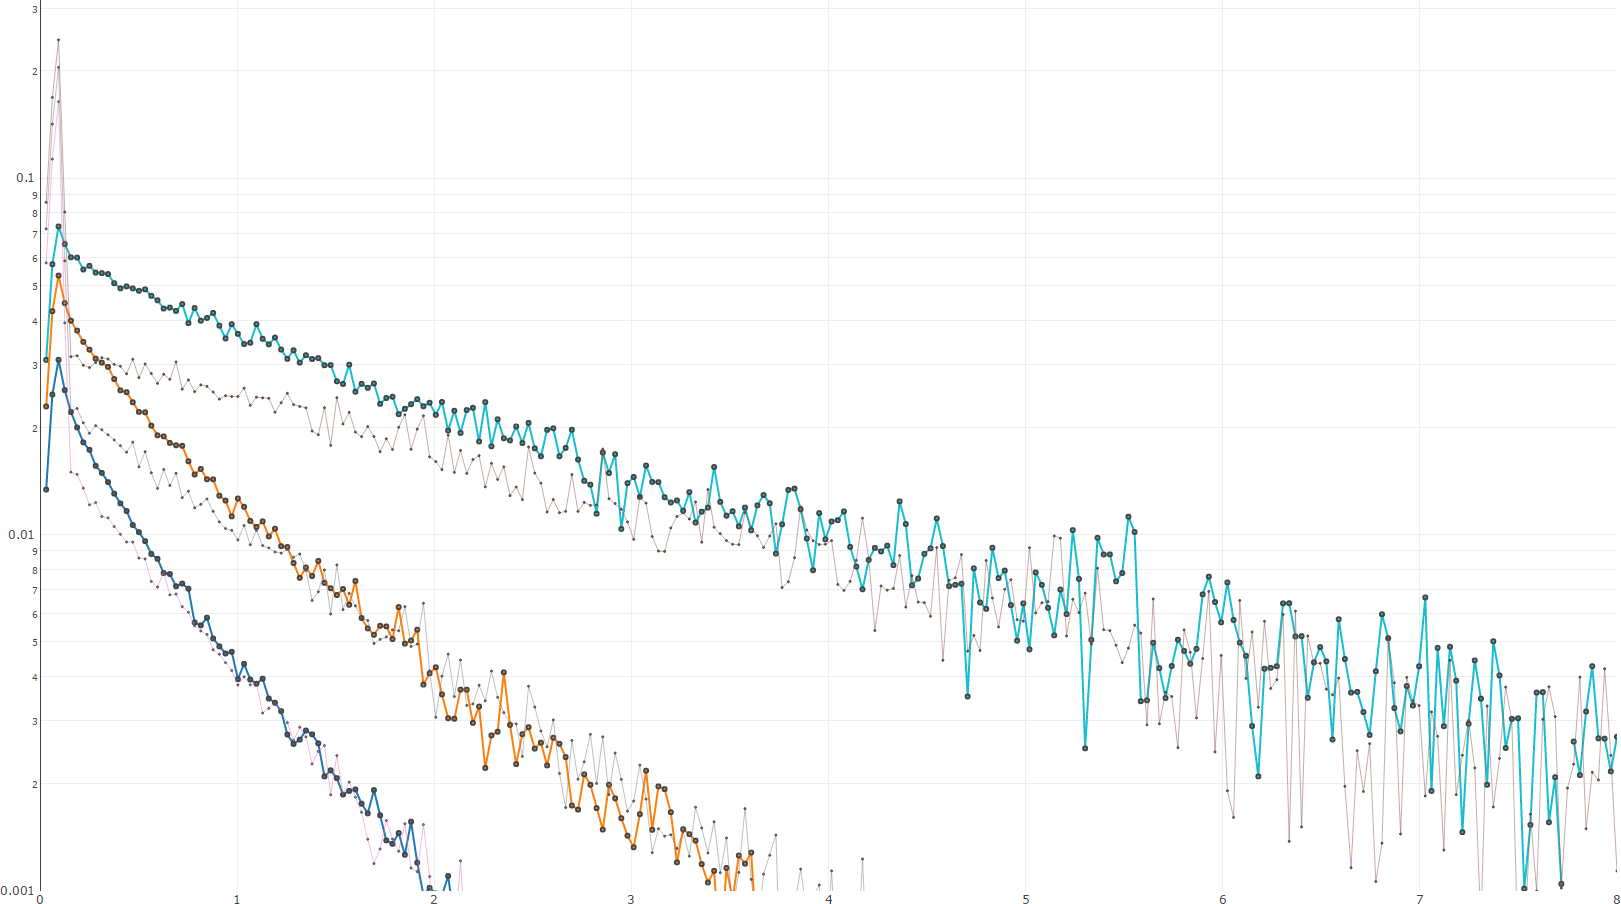
\includegraphics[width=\textwidth]{imgs/plots/burley_old_fitting}
        \caption{Original Christensen-Burley}
    \end{subfigure}
    \quad
    \begin{subfigure}{0.48\textwidth}
        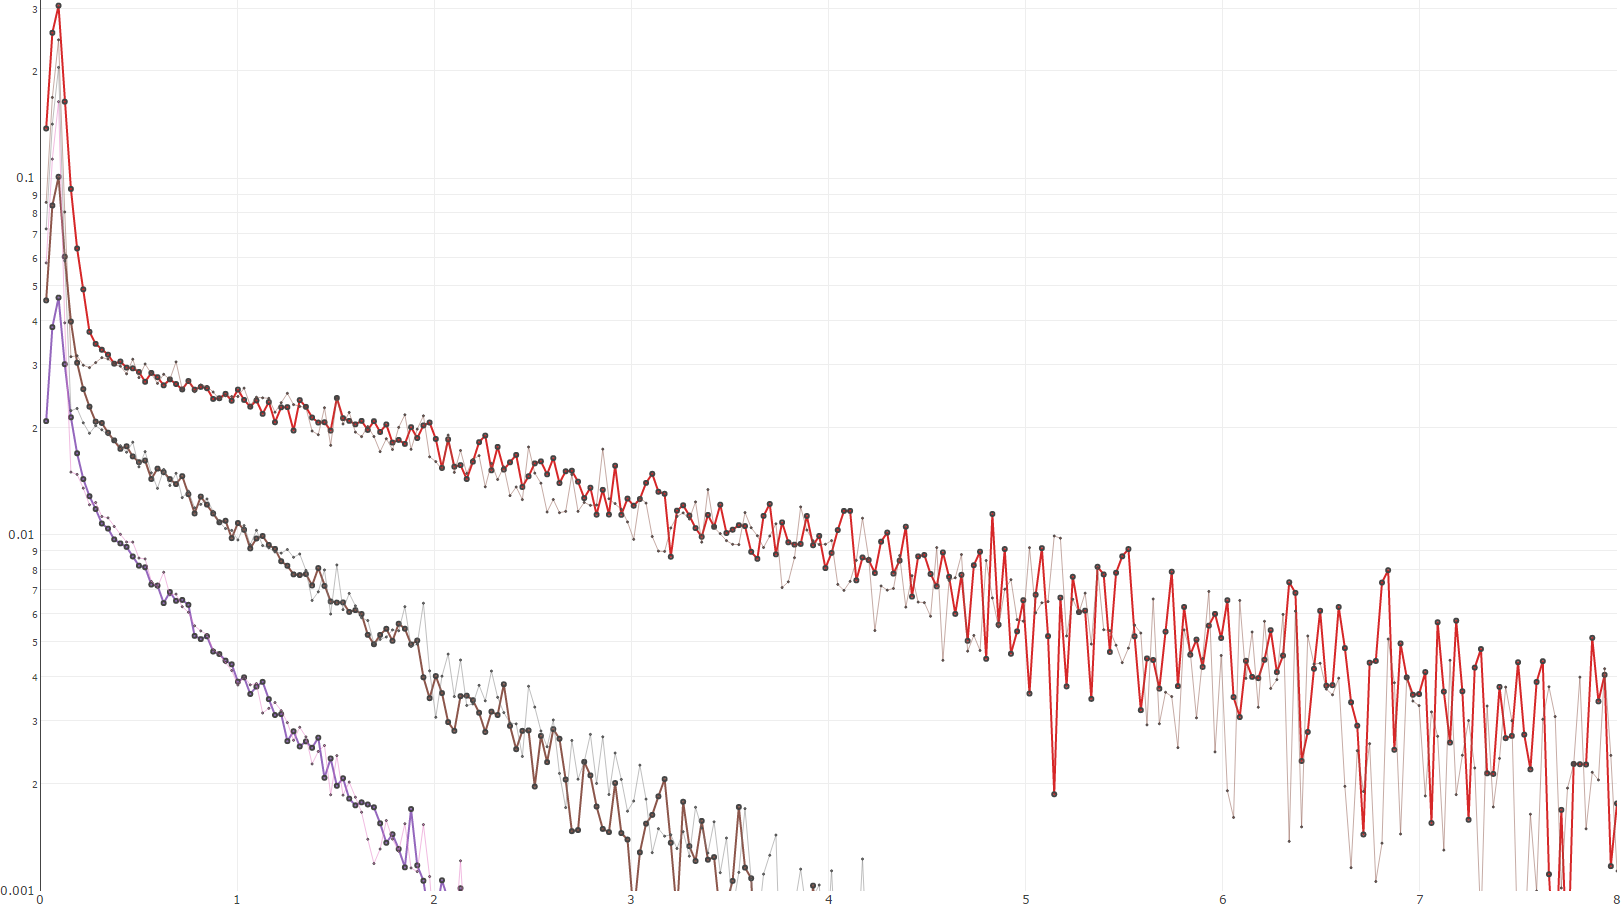
\includegraphics[width=\textwidth]{imgs/plots/burley_new_fitting}
        \caption{Proposed}
    \end{subfigure}

    \caption{Comarison between the original and proposed techniques in log-y
    scale. Monte Carlo references are inthin lines. TODO: make clear plots and
    accompany them with rendered images}
    \label{fig:burley_fitting}
\end{figure}

As we can see from the graph \ref{fig:burley_fitting}, there is a tendency for
the original model to overestimate outgoing radiant exitance in the region close
to the light source (around $x\leq=3$). This trend was observed in many
experiments with different optical properties of the material.

The proposed model has different the factorization of the exponents than the
original \gls{BSSRDF} profile. Instead of using unified parameter $s$, I propose
to split it into two factors for each of the exponent:

\begin{equation}\label{eq:burley_modified}
R_{l=1}(r) = A\dfrac{se^{-sr}+te^{-tr/3}}{8\pi r}
\end{equation}

It still allows to easily normalize the model and use the same technique for
importance sampling. The particular form of s and t is based on the original
function developed by Christensen et al., but has a linear function coefficient
to get better results.

\ldots

\section{Christensen-Burley BSSRDF profile importance sampling}
\label{section:burley_importance}
Importance sampling of the BSSRDF function is a vital part of the rendering system used in practical
applications. The short theory of importance sampling is given in the section
\ref{section:importance_sampling}. Together with the disc sampling technique described in chapter
\ref{sampling_methods} we can formulate the importance sampling problem in this context, as finding
a good distribution of the sample points around the given shading position with \gls{PDF} matching
to the above mentioned diffusion profile \ref{eq:burley} as close as possible.

Saying that, we need to derive \gls{CDF} of the profile and invert it to find the corresponding
sampling.
The \gls{CDF} of the Christensen-Burley \gls{BSSRDF} profile \ref{eq:burley} is expressed as
follows:
\[
\label{eq:burley_cdf}
CDF(R_d(r)) = \frac{\int_{0}^{r} R_d(x)2\pi xdx}{\int_{0}^{\infty} R_d(x)2\pi xdx}  = \frac{1}{A}
\int_{0}^{r} As\frac{e^{-sx}+e^{-sx/3}}{8\pi x}2\pi xdx =
1-\frac{1}{4}e^{-sr}-\frac{3}{4}e^{-\frac{sr}{3}} \] Factor $2\pi x$ in the integrand appear due to
the integration over the area of the disc in polar coordinates. And the integral in the denominator
over the whole area stands for the normalization.

Let $\xi$ be uniformly distributed random variable within the range from 0 to 1. To find the
distance from the shading position to the next sampled point $r$ according to the \ref{eq:burley},
the following equation have to be solved (inversion step):
\begin{equation}
\label{eq:inversion}
\xi=1-\frac{1}{4}e^{-sr}-\frac{3}{4}e^{-\frac{sr}{3}}
\end{equation}

This step would, in theory, result in the corresponding function $r(\xi)$ which can be used to
generate samples. But the fact that there is no analytical solution to equation
\ref{eq:inversion} makes it difficult to use in practice.
There are couple of main approaches to overcome this problem. Some of them are:
\begin{enumerate}
  \item Precompute the solution before rendering and use a lookup table with interpolation
  during the runtime
  \item Sample each of the exponential of the right side of the equation \ref{eq:burley}
  separately and combine the result
  \item Solve the equation numerically in runtime for each sample on demand
\end{enumerate}

The first mentioned precomputation approach proved be overcomplicated during implementation
without significant performance outcome \cite{Christensen:2015:ARP:2775280.2792555}. It is not
considered in this thesis. But the second and the third methods are discussed with more details
on implementation and performance results below.

\subsection{Separated sampling}
One of the possible solution to the problem of importance sampling of BSSRDF containing the sum of
two exponential functions is sampling each of the summand independently and combining the results.

Hence, two functions to be used to distribute samples:
\[
pdf_1(r)=\frac{s}{2\pi r}e^{-rs}
\]
\[
pdf_2(r)=\frac{s/3}{2\pi r}e^{\frac{-rs}{3}}
\]

Note, that additional $\frac{1}{2\pi r}$ factor is used in the implementation PDF to account for
sampling over the area of the disc. The corresponding \gls{CDF}s and sampling radii:
\[
cdf_1(r)=\int_{0}^{r} pdf_1(x) 2\pi xdx = 1-e^{-rs} \Rightarrow r_1(\xi)=-\frac{\log{\xi}}{s}
\]
\[
cdf_2(r)=\int_{0}^{r} pdf_2(x) 2\pi xdx = 1-e^{-\frac{rs}{3}} \Rightarrow
r_2(\xi)=-\frac{3\log{\xi}}{s}
\]
The linear combination of these two sampling techniques can be used to successfully integrate
Christensen-Burley BSSRDF profile. The results of the application of this method are discussed in
section \ref{importanceSamplingResults}

\subsection{Numerical root finding}
Another practical approach to find the importance sampling distribution of the \ref{eq:burley} is to
solve the full CDF equation \ref{eq:inversion} using Newton iteration for each sample. It gives
the best sampling distance for any $\xi$ with bounded error.

The constant radius of $r_0=1.0$ was taken as an initial guess. Attempts to find better
approximation for the first iteration by exponential function did not result in visible performance
improvement.

Each next step of Newton iteration the solution is improved as $r_i(\xi)=r_{i-1}-f(r)/f'(r)$ with:
\[
f(r) = 1 - \frac{1}{4}e^{-rs} - \frac{3}{4}e^{-\frac{rs}{3}} - \xi
\]
and the corresponding derivative:
\[
f'(r) = \frac{s}{4}(e^{-sr}+e^{-\frac{sr}{3}})
\]

Experiments show that for wide range of parameter $s$ values and the error tolerance of the radius
$\epsilon_r=10^{-4}$ it takes no more than 9 iterations to find the correct solution most of the
time.

\subsection{Discussion}
\label{importanceSamplingResults}
Both \emph{Separated sampling} and \emph{Numerical root finding} methods were implemented as a part
of diffusion approximation integrator and proved to converge to the same result. The figure
\ref{fig:importance_convergence} shows the root mean square error over time during convergence of
the rendering of the searchlight problem scene. The final output is shown at the image
\ref{fig:zoom_importance_sampling}.
\begin{figure}
    \centering
    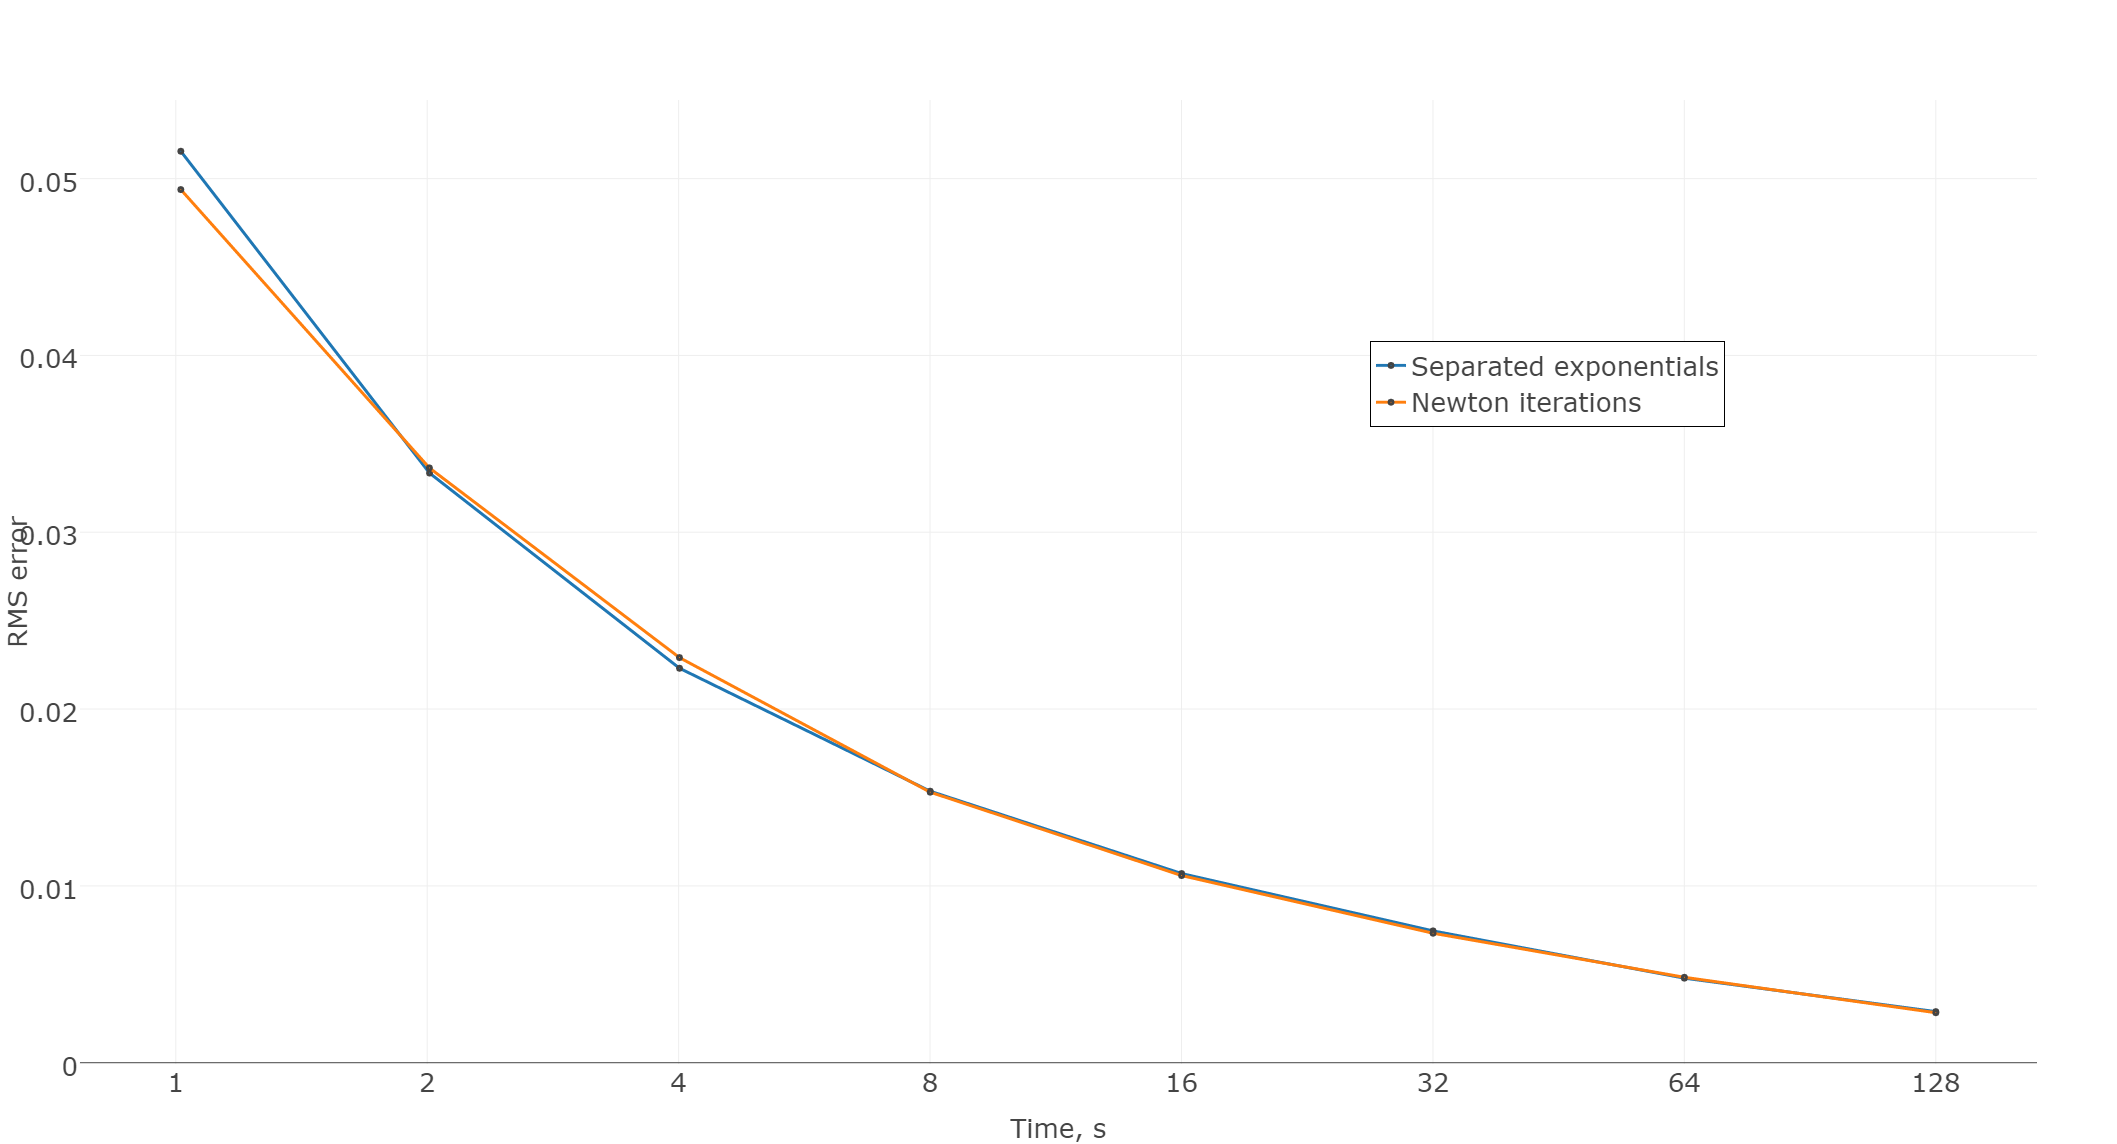
\includegraphics[width=\textwidth]{{imgs/plots/convergence_newton_exp}}
    \caption{Convergence plot over time of two importance sampling methods}
    \label{fig:importance_convergence}
\end{figure}

Both approaches result in almost identical convergence speed while measuring the error over the
whole image according to figure \ref{fig:importance_convergence}. In some cases Separated sampling
shows even better convergence. It can be observed while looking at the central part of the resulting
images after 5 seconds of rendering on figure \ref{fig:zoom_importance_sampling}.
\begin{figure}
    \centering
    \begin{subfigure}{0.3\textwidth}
        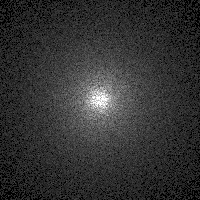
\includegraphics[width=\textwidth]{{{imgs/renders/cb_convergence/ref_exp_bigcrop_da_10.0_ds_0.1}}}
        \caption{Separated sampling}
        \label{fig:exponential_importance_sampling_zoom}
    \end{subfigure}
    \quad
    \begin{subfigure}{0.3\textwidth}
        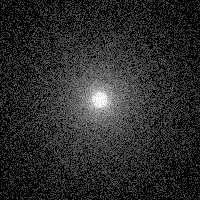
\includegraphics[width=\textwidth]{{{imgs/renders/cb_convergence/ref_newton_bigcrop_da_10.0_ds_0.1}}}
        \caption{Newton iteration}
        \label{fig:newton_importance_sampling_zoom}
    \end{subfigure}
    \caption{Equal time searchlight problem. Rendering results of the region close to the light
    source.}
    \label{fig:zoom_importance_sampling}
\end{figure}

But at the same time, this method produces unwanted fireflies in the regions far away from the light
incoming point. This effect can be seen at the figure \ref{fig:importance_sampling}. While
moderate intensity noise in the central region is reduced quite efficiently over time, the high
frequency spikes stay highly visible even after several minutes of rendering.

This is the reason why the Newton iteration was chosen as more robust and preferable importance
sampling technique for Christensen-Burley BSSRDF in out final implementation.
\begin{figure}
    \centering
    \begin{subfigure}{0.49\textwidth}
        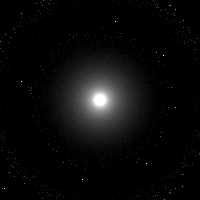
\includegraphics[width=\textwidth]{{{imgs/renders/cb_convergence/ref_exp_gamma_da_10.0_ds_0.1}}}
        \caption{Separated sampling}
        \label{fig:exponential_importance_sampling}
    \end{subfigure}
    \begin{subfigure}{0.49\textwidth}
        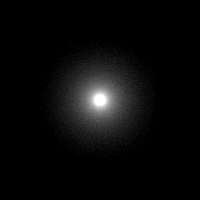
\includegraphics[width=\textwidth]{{{imgs/renders/cb_convergence/ref_newton_gamma_da_10.0_ds_0.1}}}
        \caption{Newton iteration}
        \label{fig:newton_importance_sampling}
    \end{subfigure}
    \caption{Equal time searchlight problem rendering comparison}
    \label{fig:importance_sampling}
\end{figure}

One of the possible solution of removing high frequency variance of the Separated importance
sampling is to clamp the high intense samples during rendering. This method, of course, introduces
additional bias to the final output and requires the control of the clamping threshold by the user.
But, taking into account the inherent biased nature of the Diffusion Approximation approach,
clamping may be a practical method of noise reduction with retaining lower variance in the region
close to the light.

\section{BSSRDF parametrization}
Physically based parameters $\sigma_s$ and $\sigma_a$ are used for the
description of the material appearence in the context of subsurface
scattering. The \textit{volumetric scattering albedo} coefficient
$alpha = \sigma_s / \sigma_s+\sigma_a$ is used for the same purpose while using
diffusion approximation


In contrast, BSSRDF profile for the diffusion approximation proposed by Burley
and Christensen relays on \textit{surface albedo} (diffuse surface reflectance)
$A$ of the material:



It can not be easily analytically computed at runtime out of $\sigma_s$ and $\sigma_a$. But we need it for unified parametrization on the materials independent of the rendering technique.

By rendering different materials with various oprical properties and using curve
fitting I've come up to the following expression:
\[
A(\alpha) = a + b(1- e^{-c\alpha})
\]

with parameters $a = 0.0699, b = -3.97\cdot 10^{-05}, c =-10.0$

The results from the following plot show good match for Burley profiles (thick
lines) to Monte Carlo references (thin lines) for high albedo materials (top
four curves). But there is a significant difference for low albedo materials
with approximately $A<0.3$

Note that two lower thick lines does not not correspond to lower two thin lines.
And this result is consistent with the assumptions of the diffusion theory of
the light transport in participating media.



\section{Sampling methods}

\begin{itemize}
    \item{Infinite plane disk sampling \cite{Jensen:2001:PMS:383259.383319}}
    \item{Multiresolution radiosity caching \cite{Christensen:2012:MRC:2343045.2343108}}
    \item{Bidirectional Lightcuts \cite{Walter:2012:BL:2185520.2185555}}
    \item{Improved disk sampling \cite{King:2013:BIS:2504459.2504520}}\\
    $\star$ \textit{Editors' choise}. This method was used in my implementation.
    TODO: Detailed descriprion.
\end{itemize}


